% !TeX spellcheck = es_ES
\documentclass[arial,a4paper,print]{article}

\usepackage{amsmath}
\usepackage{helvet}
\usepackage{lipsum}
\usepackage{multirow}
\usepackage{array}
\usepackage{physics}
\usepackage[version=4]{mhchem}
\usepackage{epsfig}
\usepackage{amssymb}
%\usepackage{svrsymbols}
\usepackage{siunitx}
\usepackage{graphicx}
\usepackage{subcaption}
\usepackage[labelfont=sc, font={footnotesize, singlespacing}]{caption}
\usepackage[margin=2cm]{geometry}  

\renewcommand{\familydefault}{\sfdefault}

\usepackage[spanish]{babel}
%opening
\title{Física: Selectividad 2022}
\author{tomiock}

\begin{document}
\maketitle

Los contenidos consisten en tres grandes bloques (Álgebra Lineal, Geometría y Análisis), pero el e examen tiene tan solo 6 preguntas (de las cuales se escogen 4). 

\section{Álgebra Lineal}
\subsection{Operaciones con matrices}

Las matrices tiene definida una suma, producto y producto por escalar.

Ejemplo de suma de matrices $2\cross2$:
\begin{equation*}
	\begin{pmatrix}
		a_{1} & a_{2} \\
		a_{3} & a_{4}
	\end{pmatrix} +
	\begin{pmatrix}
		b_{1} & b_{2} \\
		b_{3} & b_{4}
	\end{pmatrix} = 
	\begin{pmatrix}
		a_{1} + b_{1} & a_{2} + b_{2} \\
		a_{3} + b_{3} & a_{4} + b_{4}
	\end{pmatrix}
\end{equation*}
Tiene que tener las misma dimensiones. 

En cambio con el producto entre dos matrices, estas no tiene que tener las mismas dimensiones necesariamente. Tal solo el número de filas de una tiene que ser igual que el numero de columnas de la otra y viceversa\footnote{$(m\cross n ) \cdot (n\cross m) \mapsto (m\cross m)$}. Producto entre dos matrices: 
\begin{equation*}
\begin{pmatrix}
	a_{1 1} & \cdots & a_{1 n} \\
	\vdots & \ddots & \vdots \\
	a_{m 1} & \cdots & a_{m n}
\end{pmatrix} 
\begin{pmatrix}
	b_{1 1} & \cdots & b_{1 p} \\
	\vdots & \ddots & \vdots \\
	b_{n 1} & \cdots & b_{n p}
\end{pmatrix} \\
=
\begin{pmatrix}
	a_{11}b_{11}+ \cdots +a_{1n}b_{n1} & \cdots & a_{11}b_{1p}+ \cdots +a_{1n}b_{np} \\
	\vdots & \ddots & \vdots \\
	a_{m1}b_{11}+ \cdots +a_{mn}b_{n1} & \cdots & a_{m1}b_{1p}+ \cdots +a_{mn}b_{np}
\end{pmatrix}
\end{equation*}

O un ejemplo más claro con 2 matrices $(2\cross2)$:
\begin{equation*}
	\begin{pmatrix}
		e & f \\
		g & h
	\end{pmatrix}\begin{pmatrix}
		a & b \\
		c & d
	\end{pmatrix}
	=
	\begin{pmatrix}
		ea + fc & eb + fd\\
		ga + hc & gb + hd
	\end{pmatrix}
\end{equation*}
Se puede ver como es un producto escalar entre vectores que forman columnas y filas:
\begin{figure}[h]
	\centering
	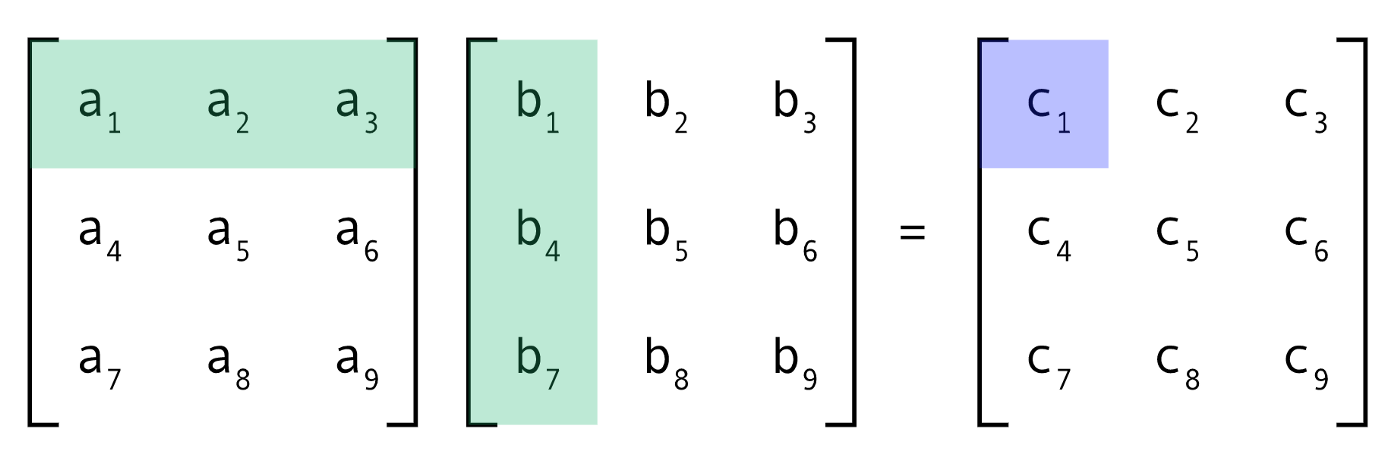
\includegraphics[width=0.5\linewidth]{producto_matrices}
	\caption{Esquema de la multipliación entre dos matrices, el producto escalar de los vectores resaltados en verde dan lugar al escalar marcado en azul. Se coge una fila de la primera matriz y una columna de la segunda. Debido a esto el producto de matrices no es conmutativo $AB\neq BA$.}
	\label{fig:productomatrices}
\end{figure}


Al multiplicar una matriz por un escalar (número), se multiplican todos los elementos de la matriz por ese escalar:
\begin{equation*}
	\begin{pmatrix}
		1 & 4  \\
		3 & 2
	\end{pmatrix}
	=
	\begin{pmatrix}
		5 \times (1) & 5\times (4)  \\
		5\times (3) & 5\times (2) 
	\end{pmatrix}
	=
	\begin{pmatrix}
		5 & 20  \\
		15 & 10
	\end{pmatrix}
\end{equation*}

\subsection{Determinantes}
El determinante es la variación el área/norma que causa una transformación lineal aplicada a una superficie/vector.

El determinantes de una matriz $(2\cross2)$ se calcula con la siguiente regla:
\begin{equation*}
	\det \begin{pmatrix} a & b \\
		c & d \end{pmatrix} = 
	\begin{vmatrix} a & b \\
		c & d \end{vmatrix} = ad - bc
\end{equation*}

Mientras que para una matriz $(3\cross3)$ se puede utilizar la expansión de Laplace\footnote{Muy útil para el cálculo de productos vectoriales entre vectores.}:
\begin{equation*}
	\begin{vmatrix}a&b&c\\ d&e&f\\ g&h&i\end{vmatrix} =
	a\begin{vmatrix}e&f\\ h&i\end{vmatrix} - b\begin{vmatrix}d&f\\ g&i\end{vmatrix} + c\begin{vmatrix}d&e\\ g&h\end{vmatrix}
\end{equation*}
Donde se puede utilizar cualquier columna o fila para expandir la matriz




\section{Geometría}
\section{Análisis}

\end{document}